\documentclass[conference]{IEEEtran}
\IEEEoverridecommandlockouts
% The preceding line is only needed to identify funding in the first footnote. If that is unneeded, please comment it out.
\usepackage{cite}
\usepackage{amsmath,amssymb,amsfonts}
\usepackage{algorithmic}
\usepackage{graphicx}
\usepackage{textcomp}
\usepackage{xcolor}
\usepackage{tikz}

\usetikzlibrary{matrix}
\def\BibTeX{{\rm B\kern-.05em{\sc i\kern-.025em b}\kern-.08em
    T\kern-.1667em\lower.7ex\hbox{E}\kern-.125emX}}
    
\begin{document}

\title{CPS843 Assignment 2}

\author{\IEEEauthorblockN{Udbhav Prasad}
\IEEEauthorblockA{\textit{500909034}}
}

\maketitle

\begin{abstract}

Second Assignment for Intro to Computer Vision (CPS843).

\end{abstract}



\section*{Part 1 - Problem 1}

Figure 1 contains the original gray scale image.

\begin{figure}[htbp]
    \centering
    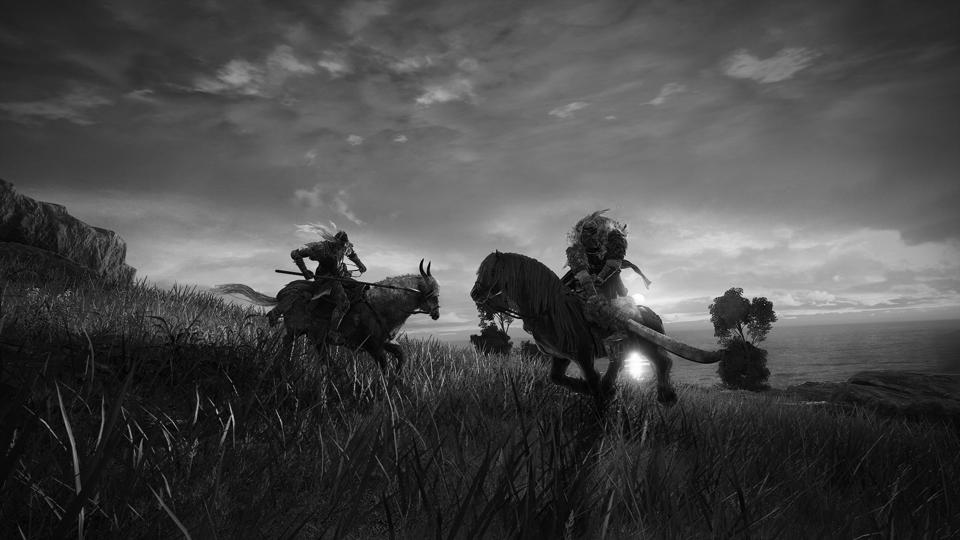
\includegraphics[width=8cm, height=4.5cm]{images/eldenring_grayscale.jpg}
    \caption{Original Gray scale Image}
\end{figure}

The more details in the detections there are, the more noise is also present, in prewitt we see that there is no false detections in the sky but other detectors capture that false edges (clouds). However, all the detections have similar edges. Noise is having alot of effect on the edges.

\subsection{Robert Edge Detection}

Figure 2 contains Robert edge detected image.

Here are the vertical/horizontal masks for Robert:

\begin{center}
\begin{tabular}{ |c|c| } 
\hline
-1 & 1 \\ \hline
\end{tabular}
\end{center}

\begin{center}
\begin{tabular}{ |c| } 
\hline
-1 & 1 \\ \hline
\end{tabular}
\end{center}

Here are the diagonal masks for Robert:

\begin{center}
\begin{tabular}{ |c|c| } 
\hline
-1 & 0 \\ \hline
0 & 1 \\ \hline
\end{tabular}
\end{center}

\begin{center}
\begin{tabular}{ |c|c|c| } 
\hline
0 & -1 \\ \hline
1 & 0 \\ \hline
\end{tabular}
\end{center}

\begin{figure}[htbp]
    \centering
    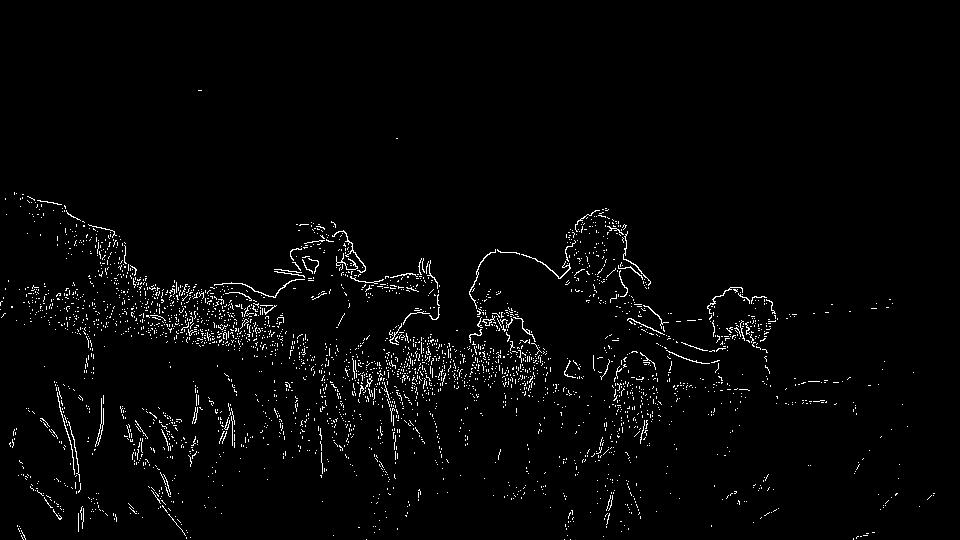
\includegraphics[width=8cm, height=4.5cm]{images/eldenring_robert.jpg}
    \caption{Robert Edge Detected Image}
\end{figure}

\subsection{Prewitt Edge Detection}

Figure 3 contains Prewitt edge detected image.

Here are the vertical/horizontal masks for Prewitt:

\begin{center}
\begin{tabular}{ |c|c|c| } 
\hline
-1 & 0 & 1 \\ \hline
-1 & 0 & 1 \\ \hline
-1 & 0 & 1 \\ \hline
\end{tabular}
\end{center}

\begin{center}
\begin{tabular}{ |c|c|c| } 
\hline
-1 & -1 & -1 \\ \hline
0 & 0 & 0 \\ \hline
1 & 1 & 1 \\ \hline
\end{tabular}
\end{center}

Here are the diagonal masks for Prewitt:

\begin{center}
\begin{tabular}{ |c|c|c| } 
\hline
0 & 1 & 1 \\ \hline
-1 & 0 & 1 \\ \hline
-1 & -1 & 0 \\ \hline
\end{tabular}
\end{center}

\begin{center}
\begin{tabular}{ |c|c|c| } 
\hline
-1 & -1 & 0 \\ \hline
-1 & 0 & 1 \\ \hline
0 & 1 & 1 \\ \hline
\end{tabular}
\end{center}

\begin{figure}[htbp]
    \centering
    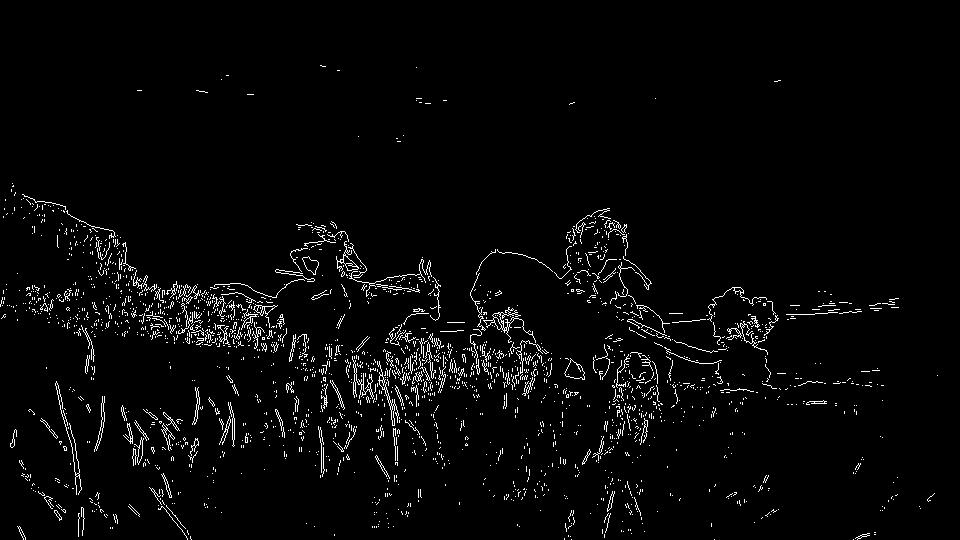
\includegraphics[width=8cm, height=4.5cm]{images/eldenring_prewitt.jpg}
    \caption{Prewitt Edge Detection Image}
\end{figure}

\subsection{Sobel Edge Detection}

Figure 4 contains Sobel edge detected image.

Here are the vertical/horizontal masks for Sobel:

\begin{center}
\begin{tabular}{ |c|c|c| } 
\hline
-1 & -2 & -1 \\ \hline
0 & 0 & 0 \\ \hline
1 & 2 & 1 \\ \hline
\end{tabular}
\end{center}

\begin{center}
\begin{tabular}{ |c|c|c| } 
\hline
-1 & 0 & 1 \\ \hline
-2 & 0 & 2 \\ \hline
-1 & 0 & 1 \\ \hline
\end{tabular}
\end{center}

Here are the diagonal masks for Sobel:

\begin{center}
\begin{tabular}{ |c|c|c| } 
\hline
0 & 1 & 2 \\ \hline
-1 & 0 & 1 \\ \hline
-2 & -1 & 0 \\ \hline
\end{tabular}
\end{center}

\begin{center}
\begin{tabular}{ |c|c|c| } 
\hline
-2 & -1 & 0 \\ \hline
-1 & 0 & 1 \\ \hline
0 & 1 & 2 \\ \hline
\end{tabular}
\end{center}

\begin{figure}[htbp]
    \centering
    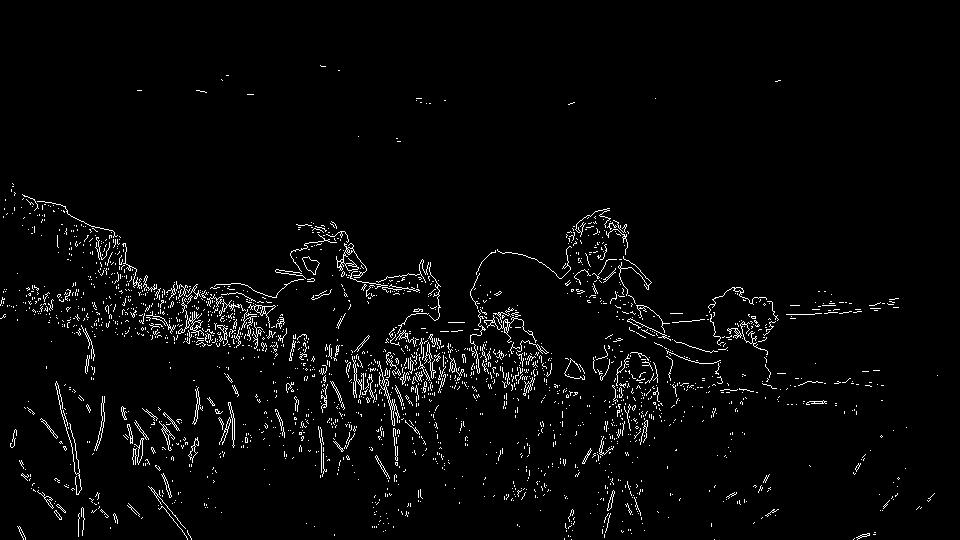
\includegraphics[width=8cm, height=4.5cm]{images/eldenring_sobel.jpg}
    \caption{Sobel Edge Detection Image}
\end{figure}

\section*{Part 1 - Problem 2}

In figure 5, we show the 1D image and the first and second order derivatives of it. We used zero padding twice to preserve the last two pixel values.

\begin{figure}
\begin{center}
\begin{tabular}{ |c|c|c| } 
\hline
f(x) & f'(x) & f''(x)\\ \hline
0 & 0 & 6\\ \hline
0 & 6 & -6\\ \hline
6 & 0 & 0\\ \hline
6 & 0 & 0\\ \hline
6 & 0 & -1\\ \hline
6 & -1 & 0\\ \hline
5 & -1 & 0\\ \hline
4 & -1 & 0\\ \hline
3 & -1 & 0\\ \hline
2 & -1 & 1\\ \hline
1 & 0 & 0\\ \hline
1 & 0 & 0\\ \hline
1 & 0 & 0\\ \hline
1 & 0 & 0\\ \hline
1 & 0 & 5\\ \hline
1 & 5 & -5\\ \hline
6 & 0 & 0\\ \hline
6 & 0 & 0\\ \hline
6 & 0 & 0\\ \hline
6 & 0 & -6\\ \hline
6 & -6 & 6\\ \hline
0 & 0 & N/A\\ \hline
0 & N/A & N/A\\ \hline
\end{tabular}
\caption{1D Image 1st and 2nd order derivatives with zero padding}
\end{center}
\end{figure}

\section*{Part 1 - Problem 3}

\begin{itemize}
  \item \textbf{Step 1:} You blur the image with Gaussian filter.
  \item \textbf{Step 2:} Subtract the original image with the blurred image and obtain the mask.
  \item \textbf{Step 3:} Add the mask to the original image with the mask you obtained multiplied by a constant k value. What you obtain is the sharpened image.
\end{itemize}

With k=1, we obtain this image:

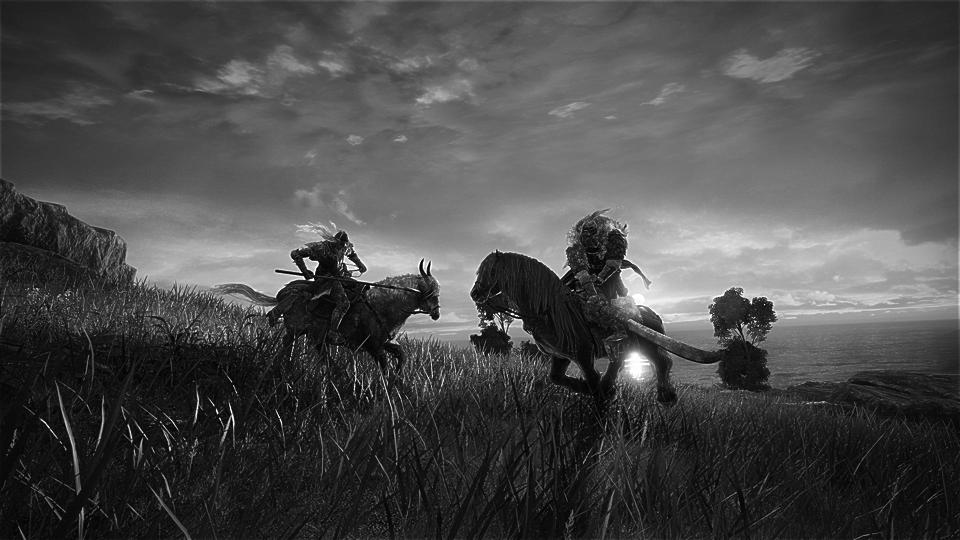
\includegraphics[width=8cm, height=4.5cm]{images/eldenring_sharpen_1.jpg}

With k=5, we obtain this image:

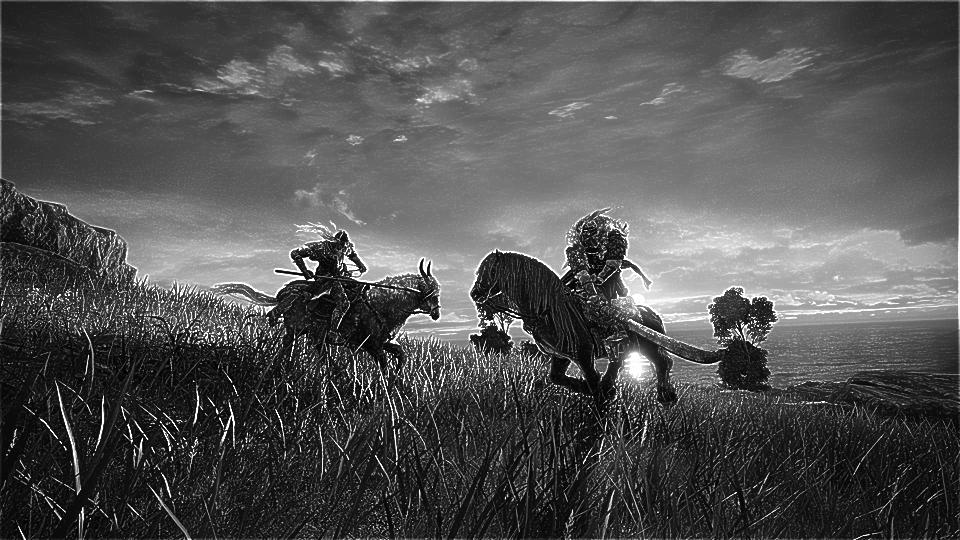
\includegraphics[width=8cm, height=4.5cm]{images/eldenring_sharpen_5.jpg}

With k=1, the image appears to have more sharpened edges but with k=5, it has very large differences in the edges. k=5, the images appears very bold in the image, this is because we add higher intensity of the mask.

\section*{Part 1 - Problem 4}

In figure 6 and figure 7, we add and remove Gaussian noise, the results are very nice. Average filter applies a smoothing/blurring effect on the image. Gaussian filter removes the noise from the image and creates a more even image.

\begin{figure}
    \begin{tabular}{c}
        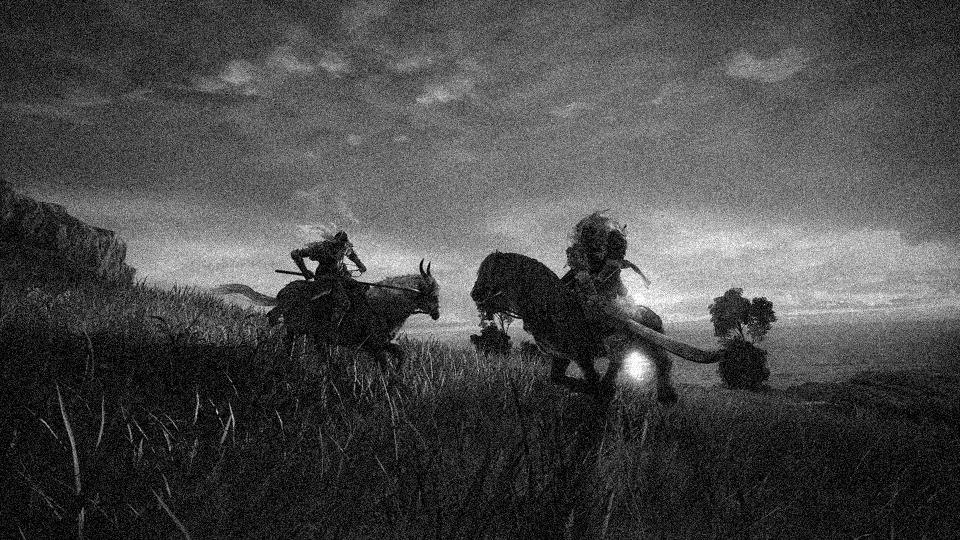
\includegraphics[width=8cm]{images/eldenring_noise_1.jpg} \\
        (a) Gaussian Noise \\[6pt]
        mu=0 var=0.005 \\[6pt]
        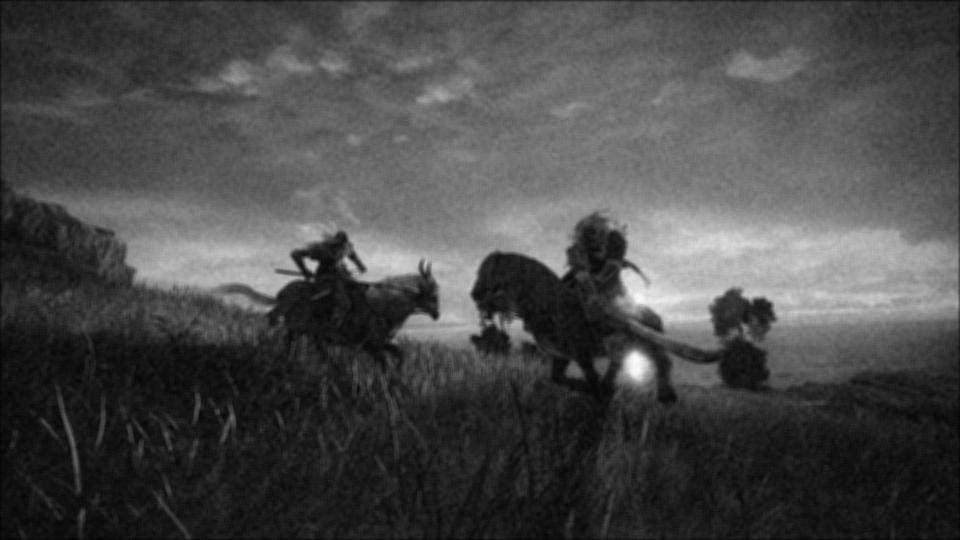
\includegraphics[width=8cm]{images/eldenring_average_1.jpg} \\
        (c) Medium Filter 5x5 \\[6pt]
        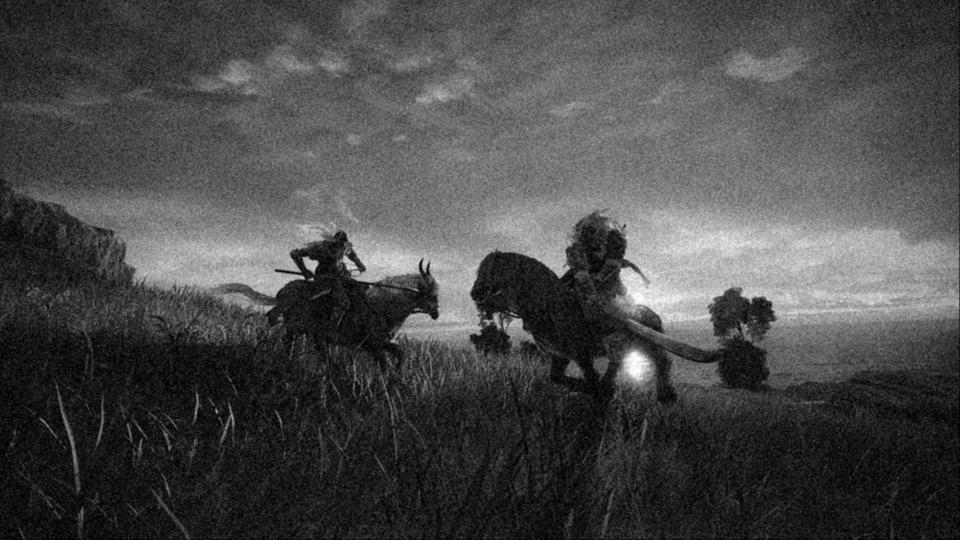
\includegraphics[width=8cm]{images/eldenring_g_1.jpg} \\
        (e) Gaussian Filter 10x10 \\[6pt]
    \end{tabular}
    \caption{Problem 4, First Image Noise Removal}
\end{figure}

\begin{figure}
    \begin{tabular}{c}
        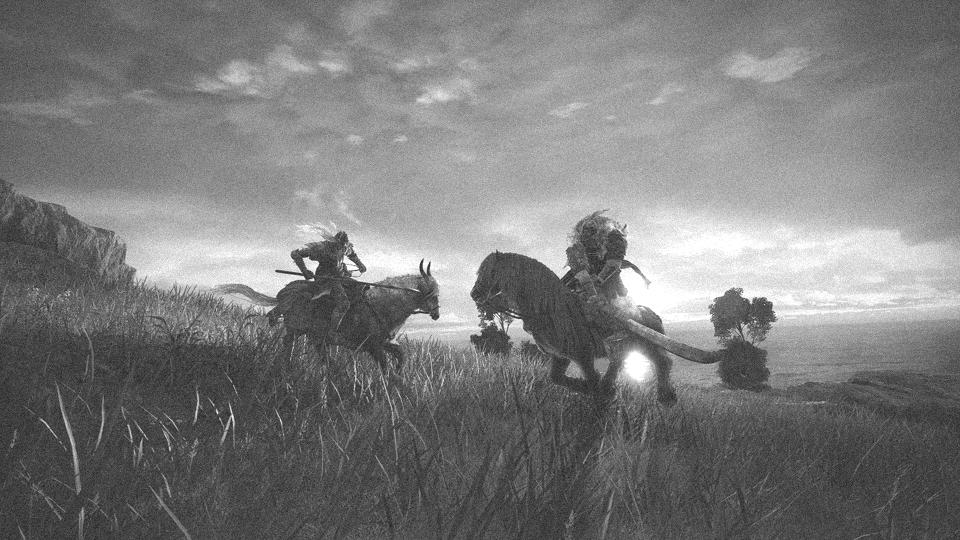
\includegraphics[width=8cm]{images/eldenring_noise_2.jpg} \\
        (b) Gaussian Noise \\[6pt]
        mu=0.2 var=0.001 \\[6pt]
        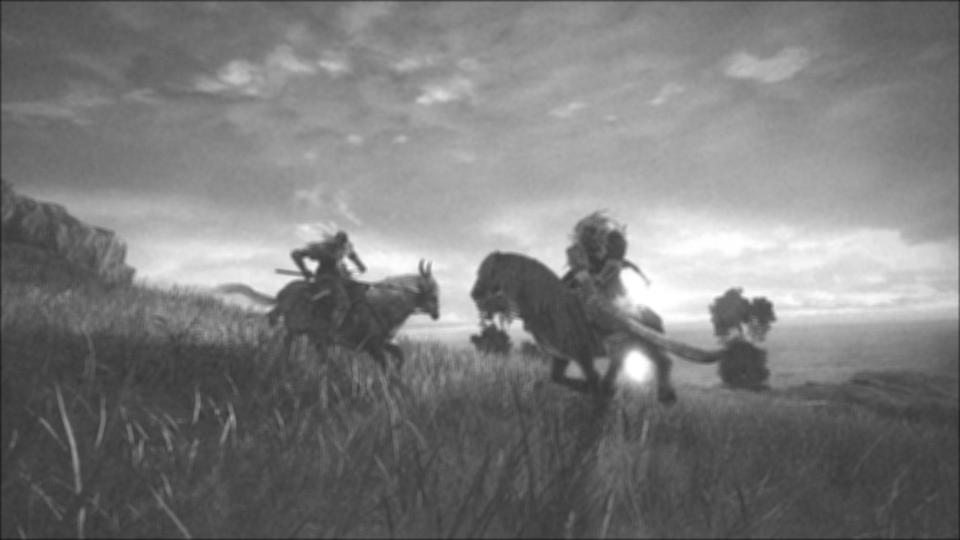
\includegraphics[width=8cm]{images/eldenring_average_2.jpg} \\
        (c) Medium Filter 5x5 \\[6pt]
        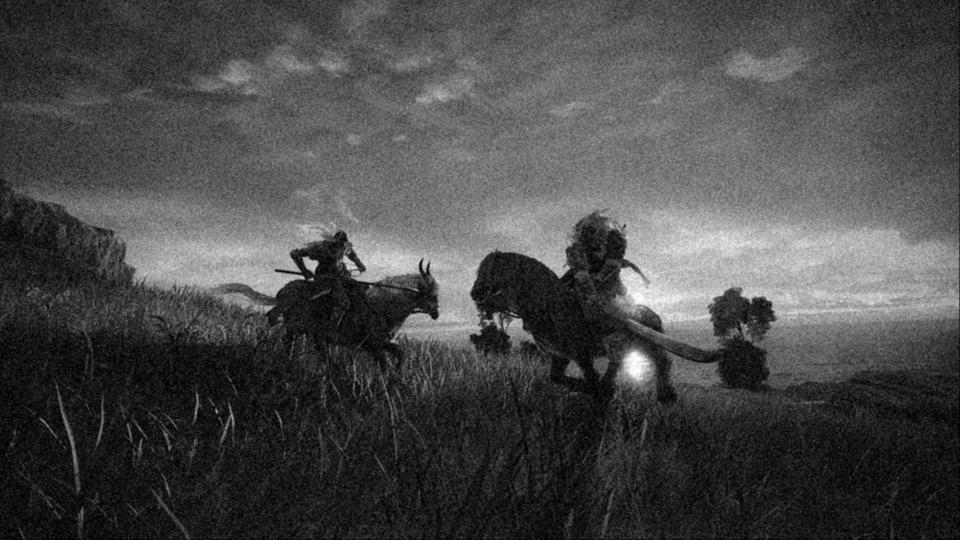
\includegraphics[width=8cm]{images/eldenring_g_2.jpg} \\
        (e) Gaussian Filter 10x10 \\[6pt]
    \end{tabular}
    \caption{Problem 4, Second Image Noise Removal}
\end{figure}

\section*{Part 1 - Problem 5}

Equations for First order derivative of f(x, y):

\begin{equation}
\frac{\partial f(x, y)}{\partial x} = f(x+1, y) - f(x, y)
\end{equation}

\begin{equation}
\frac{\partial f(x, y)}{\partial y} = f(x, y+1) - f(x, y)
\end{equation}

Equation for Laplacian of a 2D image:

\begin{equation}
\nabla^2 f = \frac{\partial f^2(x, y)}{\partial x^2} + \frac{\partial f^2(x, y)}{\partial y^2}
\end{equation}

Image is:

\begin{center}
\begin{tabular}{ |c|c|c|c| } 
\hline
0 & 2 & 5 & 7 \\ \hline
2 & 5 & 7 & 3\\ \hline
5 & 6 & 3 & 1\\ \hline
5 & 2 & 1 & 0 \\ \hline
\end{tabular}
\end{center}

First order with respect to x:

\begin{center}
\begin{tabular}{ |c|c|c|c| } 
\hline
2 & 3 & 2 & -7 \\ \hline
3 & 2 & -4 & -3\\ \hline
1 & -3 & -2 & -1\\ \hline
-3 & -1 & -1 & 0 \\ \hline
\end{tabular}
\end{center}

First order with respect to y:

\begin{center}
\begin{tabular}{ |c|c|c|c| } 
\hline
2 & 3 & 2 & -4 \\ \hline
3 & 1 & -4 & -2\\ \hline
0 & -4 & -2 & -1\\ \hline
-5 & -2 & -1 & 0 \\ \hline
\end{tabular}
\end{center}

Mask for Laplacian:

\begin{center}
\begin{tabular}{ |c|c|c| } 
\hline
0 & 1 & 0\\ \hline
1 & -4 & 1\\ \hline
0 & 1 & 0\\ \hline
\end{tabular}
\end{center}

Image after Laplacian and Normalization:

\begin{center}
\begin{tabular}{ |c|c|c|c| } 
\hline
4/9 & 2/9 & -4/9 & -20/9 \\ \hline
2/9 & -3/9 & -12/9 & 3/9\\ \hline
-7/9 & -9/9 & 3/9 & 2/9\\ \hline
-13/9 & 4/9 & 1/9 & 2/9 \\ \hline
\end{tabular}
\end{center}

Laplacian is done with mask by element wise multiplication then summation then normalization with the neighbourhood of each pixel:

Example for top left pixel: ((0)(0) + (0)(1) + (0)(0) + (0)(1) + (0)(-4) + (2)(1) + (0)(0) + (2)(1) + (5)(0))/9 = 4/9

\section*{Part 2}

Description of image enhancement algorithm:

An overview is that we invert the image then perform the haze removal algorithm then invert the image again to get the output.

The steps:

\begin{itemize}
  \item \textbf{Step 1:} Enhance Low Light Image using Dehazing Algorithm:
  
  In this step, we invert the image, apply haze removal algorithm (imreadhaze) and invert it again to obtain the enhanced low light image.
  
  \item \textbf{Step 2:} Improve Results Further Using imreducehaze Optional Parameters:
  
  In this step, we use same method as step 1 but improve on the method with better parameters: with contrast enhancement and boost per pixel.
  
  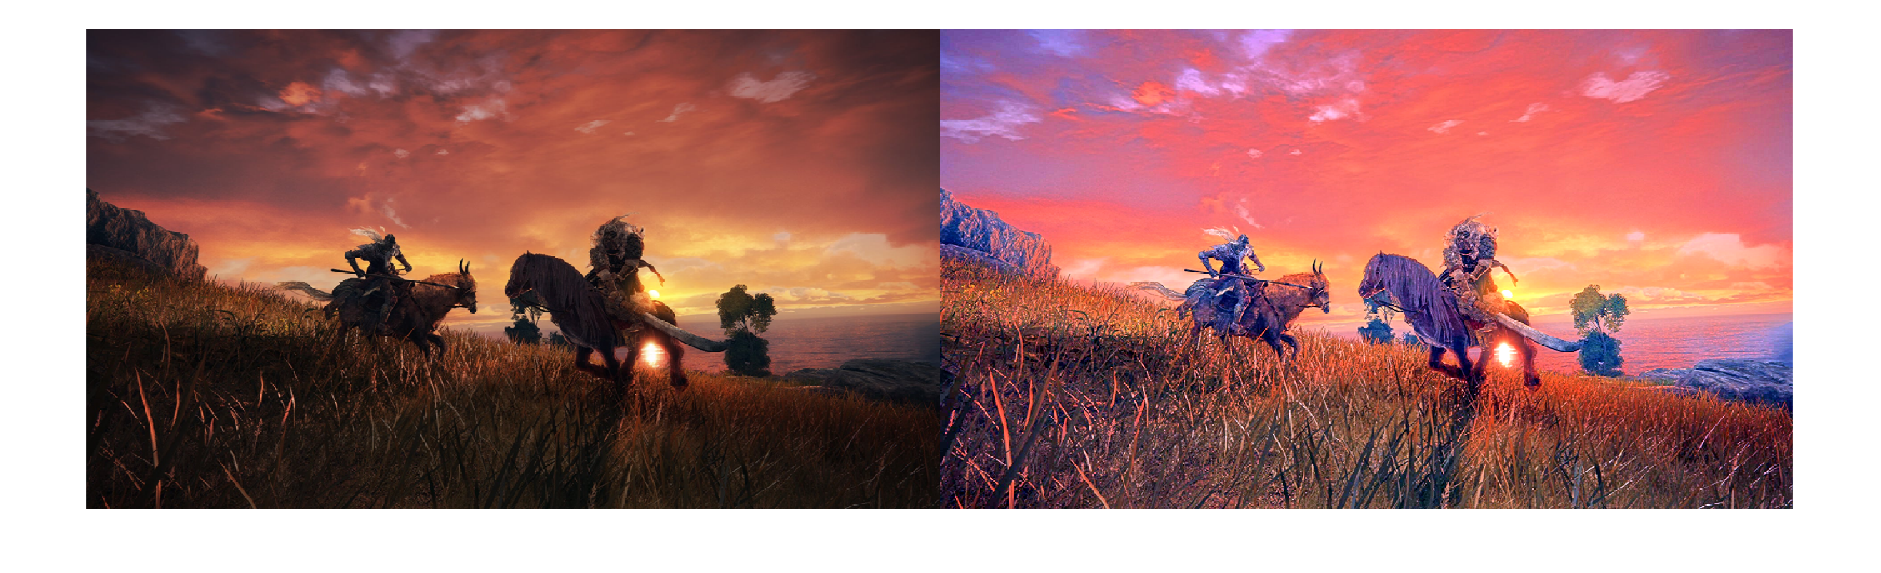
\includegraphics[width=8cm]{images/step2.png}
  
  \item \textbf{Step 3:} Another Example of Improving Poorly Lit Image:
  
  In this step, we perform haze reduction algorithm on another image with just improvement of contrast enhancement.
  
  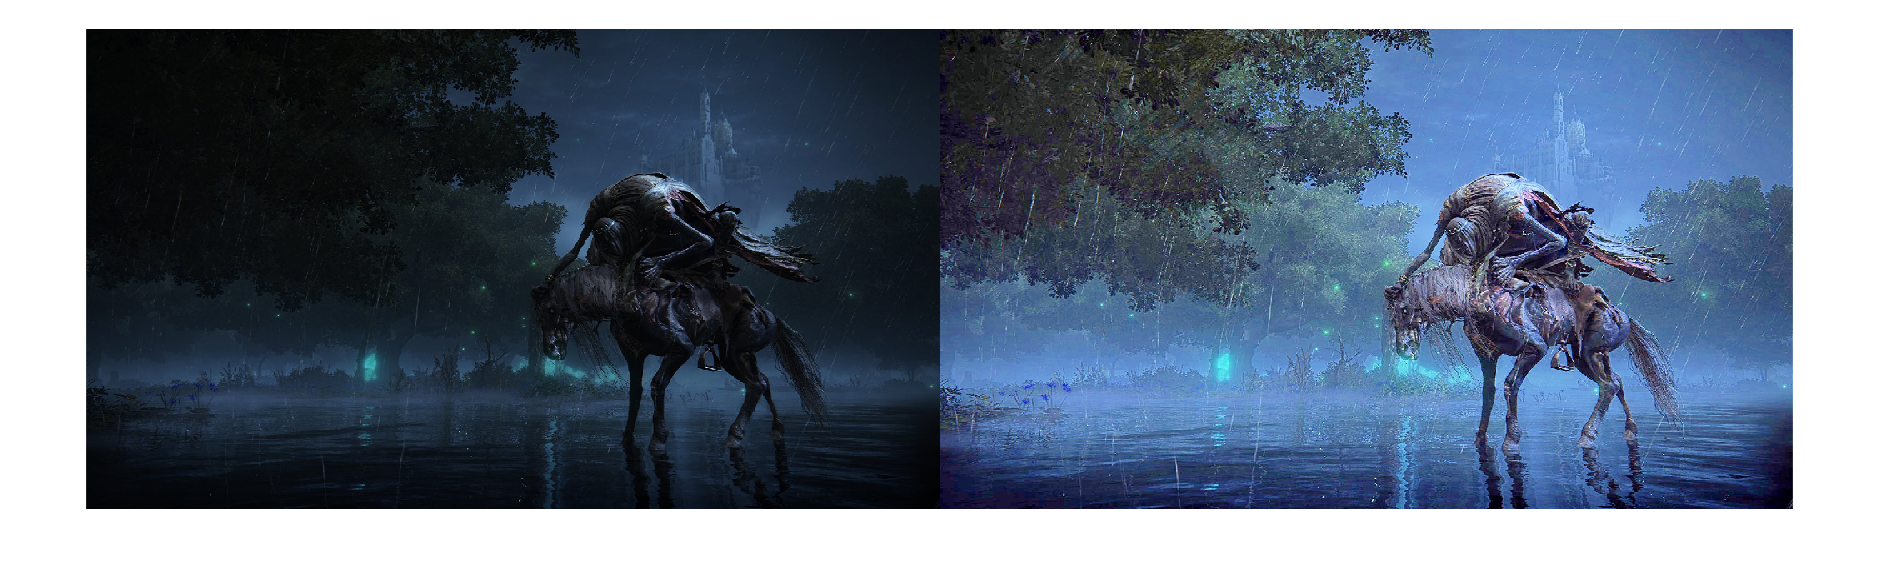
\includegraphics[width=8cm]{images/step3.png}
  
  \item \textbf{Step 4:} Reduce Color Distortion by Using Different Color Space:
  
  We perform the same steps as step 3 but we convert to L*a*b colorspace before the process and convert back to rgb after the process. Here we get better results.
  
  \item \textbf{Step 5:} Improve Results Using Denoising:
  
  Low light images have a lot of noise hence enhancing them increases noise. After the process we use imguidedfilter to remove noise from the image.
  
  \item \textbf{Step 6:} Estimate Illumination Map:
  
  In this step we compare the image after enhancing with the color map.
  
\end{itemize}

\section*{Code for Assignment 2}

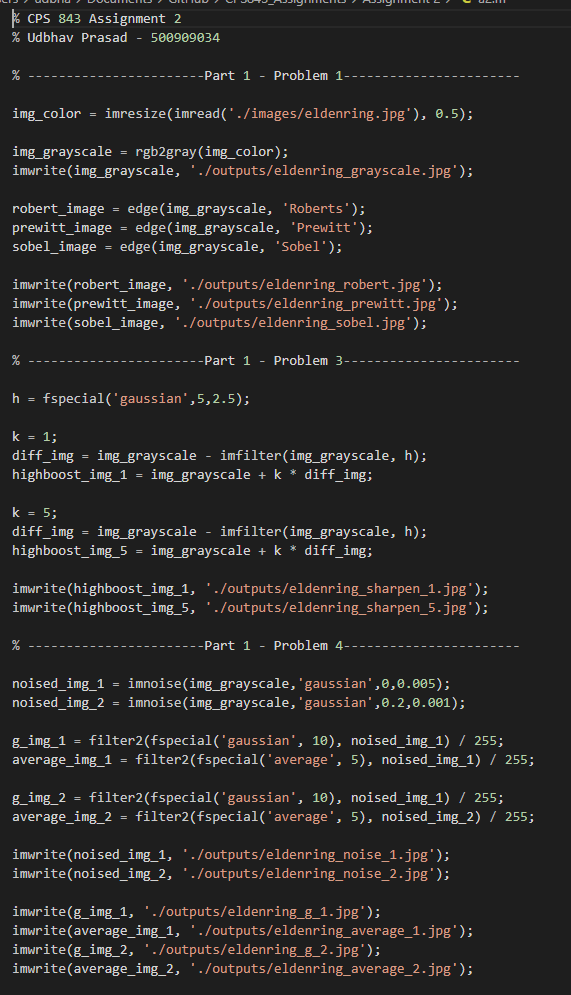
\includegraphics[width=8cm]{images/a2_code.png}

\begin{thebibliography}{00}
\bibitem{b1} Code for this assignment at ./a2.m
\bibitem{b2} Assignment source code: \href{https://github.com/UdbhavPrasad072300/CPS843-Assignments}
\end{thebibliography}

\end{document}
